\documentclass[border=7pt]{standalone}
\usepackage{tikz}
\begin{document}
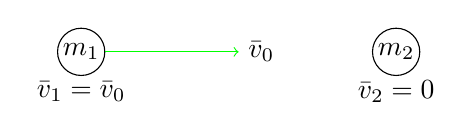
\begin{tikzpicture}
  \draw (1,0) circle [radius=0.3] node {$m_1$};
  \draw [green, ->] (1.3,0) -- (3,0) node [black, right] {$\bar{v}_0$};
  \node (c) at (1,-0.5){$\bar{v}_1=\bar{v}_0$};
  \draw (5,0) circle [radius=0.3] node {$m_2$};
  \node (c) at (5,-0.5){$\bar{v}_2=0$};
\end{tikzpicture}
\end{document}
